\section{Jadro pr\'ace}

Začnime rovnicou

\begin{equation}\label{r:2}
\frac{\ud^2y}{\ud t^2}+\frac{\ud y}{\ud t}+y =0, \qquad y(0)=1, \quad
y\,'(0)=15.
\end{equation}

Grafický priebeh riešenia tejto rovnice vidíme na Obrázku \ref{o:2}.

\begin{figure}[ht!]
\centering
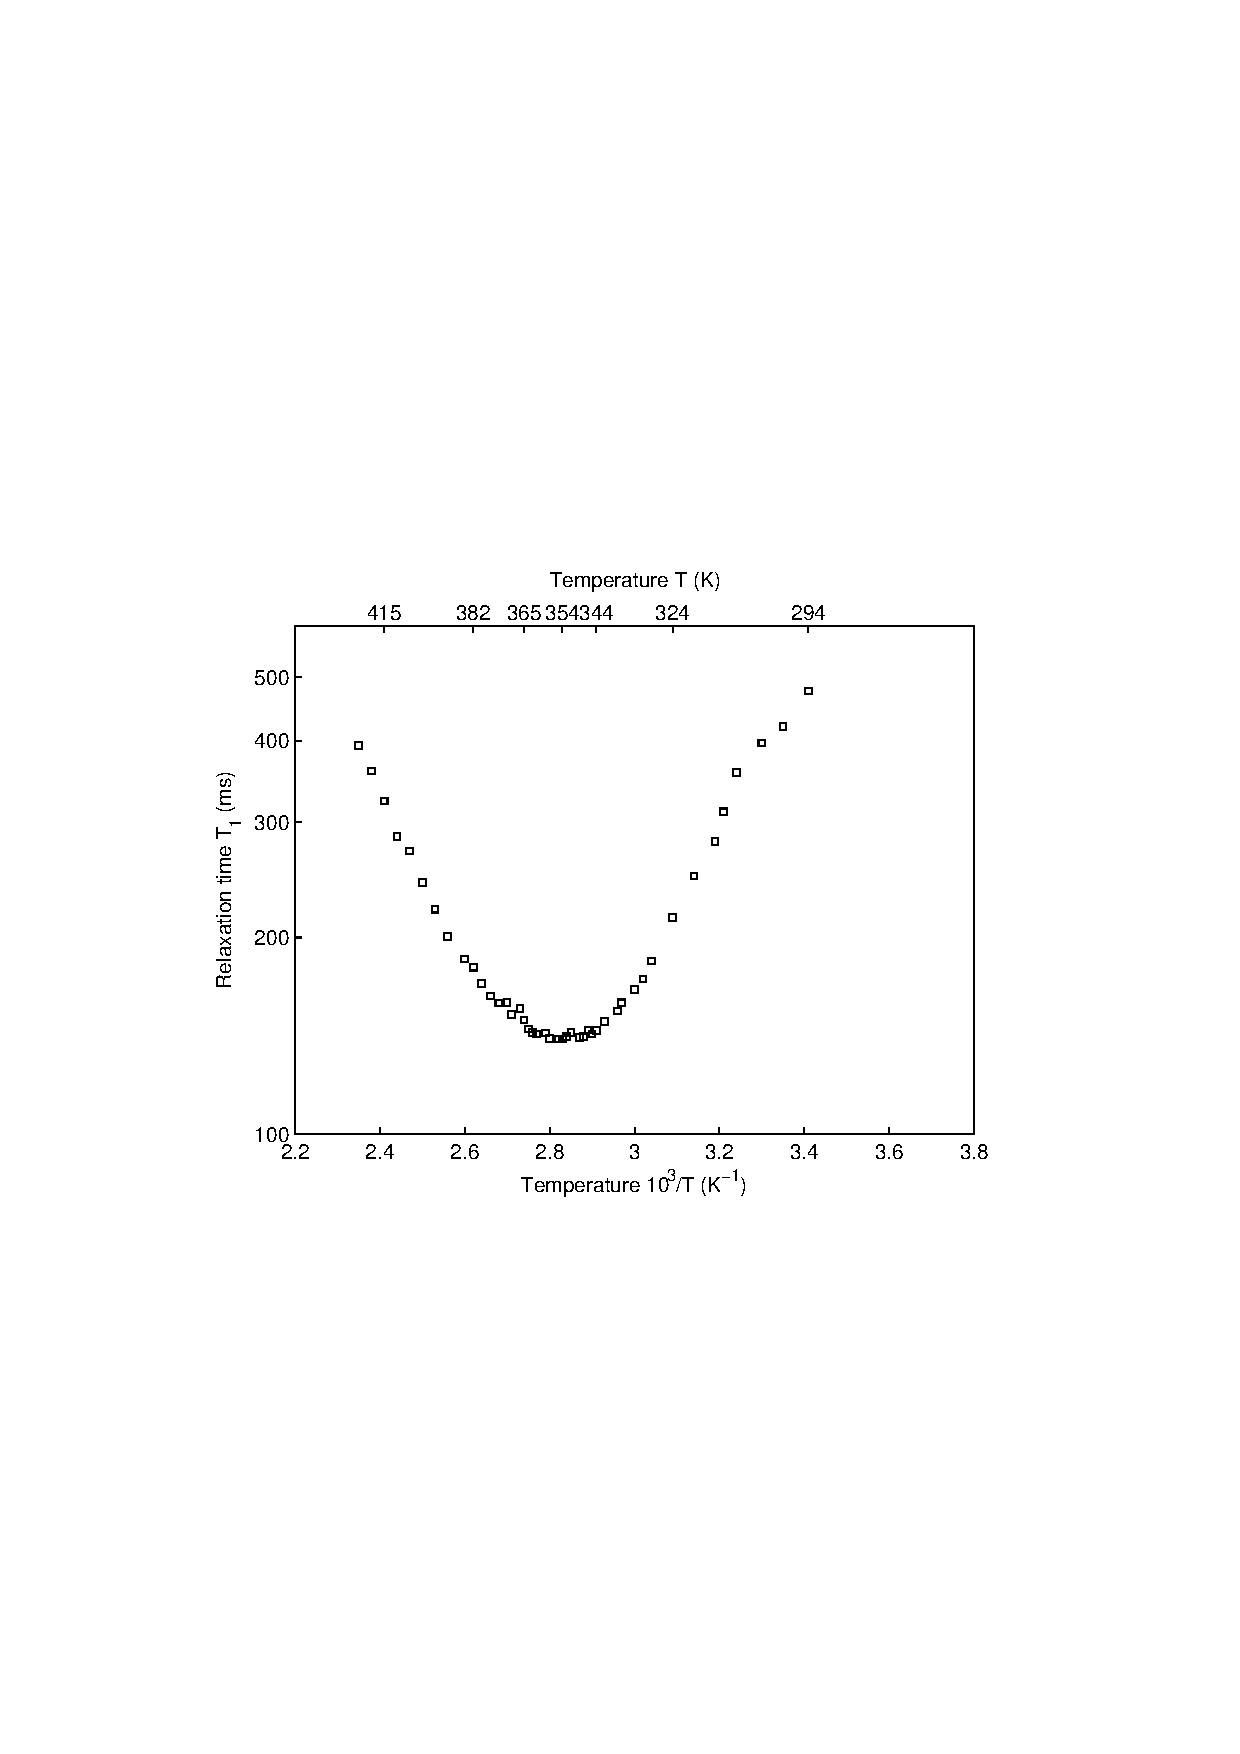
\includegraphics[width=.6\textwidth,angle=0]{relaxcas.pdf}
\caption{Teplotná závislosť\/ spinovo-mriežkového relaxačného
času}\label{o:3}
\end{figure}

%\tabcolsep=3pt % sirka stlpcov
%\renewcommand{\arraystretch}{1.2} % riadkovanie
\begin{table}[ht!]
\centering
\caption{Parametre získané z~meraní spinovo-mriežkových relaxačných
časov $T_1$}\label{t:2}
\medskip
\newcolumntype{d}{D{,}{,}{-1}}
\begin{tabular}{||c||d|d|d|d|d||}
\hhline{|t:==t:==:==:t|}
\multicolumn{1}{||c||}{}&\multicolumn{1}{c|}{PP --
01}&\multicolumn{1}{c|}{PP -- 05}&\multicolumn{1}{c|}{PP --
10}&\multicolumn{1}{c|}{PP -- 16}&\multicolumn{1}{c||}{PP -- 22} \\
\hhline{|:==:==:==:|}
C $\cdot 10^8$~(s$^{-2}$) & 10,1 & 10,0 & 11,0 & 9,2 & 8  \\
\hhline{||-|-|-|-|-|-||}
$\tau_0 \cdot 10^{-14}$~(s) & 2,63 & 1,44 & 0,95 & 2,21 & 10,83  \\
\hhline{||-|-|-|-|-|-||}
$E_{\text a}$~(kJ) & 34,26 & 8,33 & 39,76 & 37,31 & 31,86  \\
\hhline{||-|-|-|-|-|-||}
$T_{\min}$~(K) & 354 & 367 & 367 & 369 & 367  \\
\hhline{||-|-|-|-|-|-||}
$T_{1\min}$~(ms) & 141 & 160 & 157 & 175 & 181  \\
\hhline{||-|-|-|-|-|-||}
$\Delta M_2$~(Gs$^2$) & 5,49 & 5,66 & 5,16 & 5,09 & 5,02  \\
\hhline{|b:==b:==:==:b|}
\end{tabular}
\end{table}

